\chapter{Basic Definitions}

In this chapter basic definitions necessary in the following chapters are placed. The definitions are taken from \cite{RepAndConsistentAnswer, QueryXML, ImprovingXML}.


\section{XML Trees and DTDs}
\begin{define}[Tree]
Being given an alphabet of nodes $\mathbb{N}$ and an alphabet of node labels $\Sigma$, a {\sl tree} $T$ over $\mathbb{N}$ and $\Sigma$ is a tuple $(r_T, N_T, E_T, \lambda_T)$, where $N_T \subseteq \mathbb{N}$ is the set of nodes, $\lambda_T : N_T \to \Sigma$ is a node labelling function, $r_T \in N_T$ is the distinguished root of $T$, and $E_T \subseteq N_T \times N_T$ is a set of edges such that starting from any node $n_i \in N_T$ it is possible to reach any other node $n_j \in N_T$, walking through a sequence of edges $e_1,\dots,e_k$ which are connected and acyclic.\qed
\end{define}

\noindent Let us also denote the set of leaf nodes as $Leaves(T)$ and the set of trees defined over an alphabet of node labels $\Sigma$ as $T_\Sigma$.

\begin{define}[XML Tree]\label{xmlTree}
{\sl XML tree} is a pair $XT=\langle T,\delta \rangle$, where:
\renewcommand{\labelenumi}{\roman{enumi})}
	\begin{enumerate}
		\item $T = (r, N, E, \lambda)$ is a tree from $T_{\tau\cup\alpha\cup\{S\}}$, where $\tau$ is a tag alphabet, $\alpha$ is an attribute name alphabet and $S$ is a symbol not belonging to $\tau\cup\alpha$ (representing \texttt{\#PCDATA} content of elements)$;$
		\item given a node $n$ of $T$, $\lambda(n) \in \alpha \cup \{S\} \Leftrightarrow n \in Leaves(T);$
		\item $\delta : Leaves(T) \rightarrow Str$ where $Str$ is a string alphabet is a function associating a (string) value to every leaf of $T$.
	\end{enumerate}\qed
\end{define}

\begin{example}\label{example1ref}
Consider the following XML document representing a collection of books. Its graphical representation as an XML tree is in Fig. \ref{example1}.
\begin{verbatim}
<bib>
  <book>
    <written_by>
      <author ano="A1">
        <name>John Writer</name>
      </author>
      <author ano="A1">
        <name>Eric Seller</name>
      </author>
    </written_by>
    <title>Some title</title>
  </book>
  <book>
    <written_by>
      <author ano="A2">
        <name>Adam Publisher</name>
      </author>
    </written_by>
    <title>Some title 2</title>
  </book>
</bib>
\end{verbatim}

The nodes of an XML tree have a label denoting the tag name of the element and unique element identifier in brackets. Leaf nodes are either an attribute or the textual content of an element. The label of a textual node contains string contained inside of element and unique element identifier. The label of an attribute node contains in addition to textual node the name of the attribute.\qed
\end{example}

\begin{figure}[h]
    \centering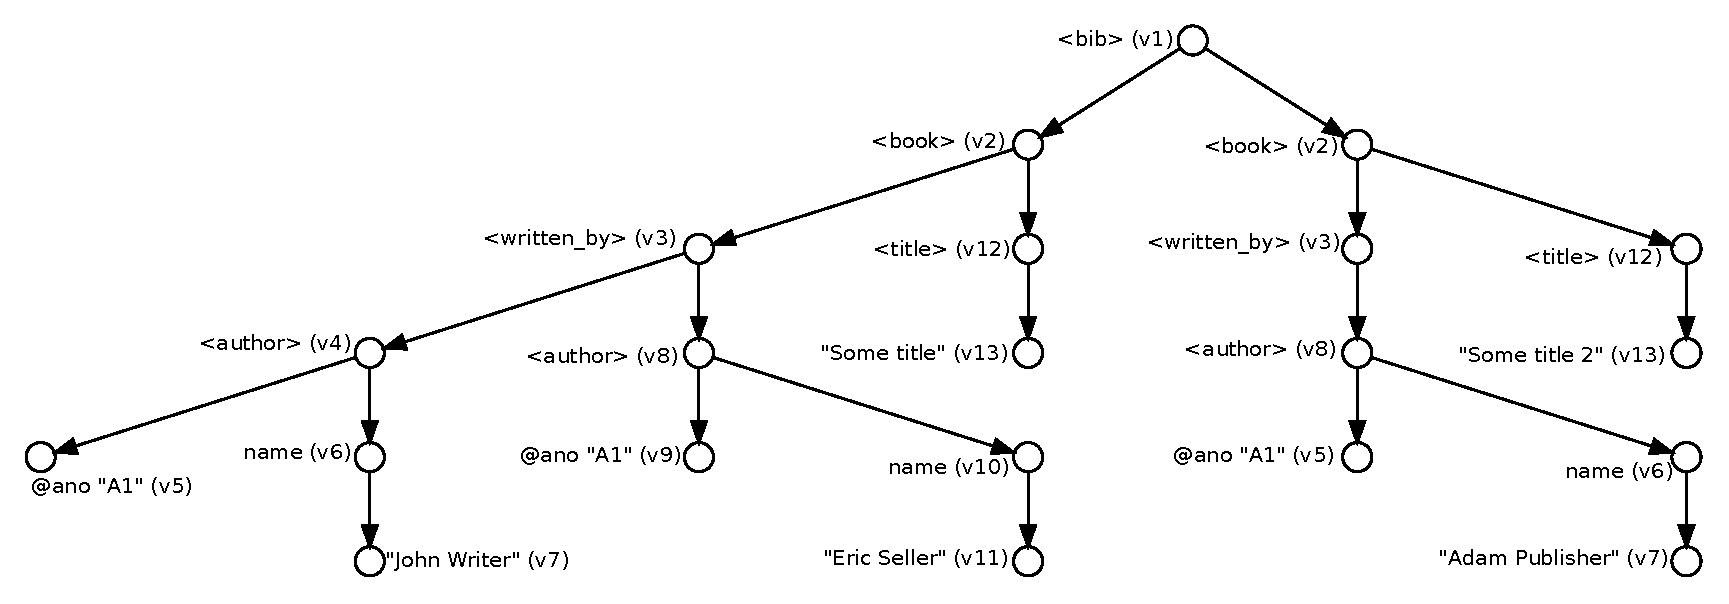
\includegraphics[width=\textwidth]{example1-new}
	\caption{An XML Tree} \label{example1}
\end{figure}

\begin{define}[DTD]\label{dtdDef}
{\sl DTD} is a tuple $D = (\tau, \alpha, P, R, rt)$ where:
\renewcommand{\labelenumi}{\roman{enumi})}
\begin{enumerate}
	\item $\tau$ and $\alpha$ are of the same definition as in the \emph{XML tree}
    \item $P$ is the set of \emph{element type definitions}
    \item $R$ is the set of \emph{attribute lists}
    \item $rt \in \tau$ is the tag of the document root element.
\end{enumerate}
\qed
\end{define}

\begin{define}[Path Expression]
A {\sl path expression} is an expression of the form $p = ('/' | '//')s_1 \dots ('/'|'//')s_m$ where $s_1, \dots, s_{m-1} \in \tau$, and $s_m \in \tau \cup \alpha \cup \{S\}$.\qed
\end{define}

\begin{define}[Path]
{\sl Path} p on a DTD $D = (\tau, \alpha, P, R, rt)$ is a sequence $p = s_1, \dots, s_m$ of symbols in $\tau \cup \alpha \cup \{S\}$ such that:
\renewcommand{\labelenumi}{\roman{enumi})}
	\begin{enumerate}
		\item $s_1=rt$;
		\item for each $i$ in $2..m-1$, $s_i \in \tau$ and $s_i$ appears in the element type definition of $s_{i-1}$;
		\item $s_m \in \alpha \Rightarrow s_m$ appears in the attribute list of $s_{m-1}$;
		\item $s_m \in \tau \cup \{S\} \Rightarrow s_m$ appears in the element type definition of $s_{m-1}$.
	\end{enumerate}\qed
\end{define}

As we have defined a \emph{path} on a DTD $D$, let us denote $paths(D)$ as the set of all paths which can be defined on a DTD $D$. Also, another important notion is $p(XT)$ (or $\{[\![p]\!]\}$), which is the set of nodes from XML tree $XT$ conforming to DTD $D$, which can be reached by the path $p \in paths(D)$, starting from the root of $XT$. The set of nodes reachable from a node $v$ following path $p$ is denoted as $\{v[\![p]\!]\}$. When there is only one node in $\{v[\![p]\!]\}$, we use $v[\![p]\!]$ to denote this node. Moreover, let $XT.p$ denote the \emph{answer} of the path $p$ applied on $XT$ that is:
\begin{itemize}
	\item if $p \in EPath(D)$, where $EPath(D)$ denotes the set of the paths whose last symbol denotes an element, then $XT.p = p(XT)$
	\item if $p \in StrPath(D)$, where $StrPath(D)$ denotes the set of paths whose last symbol denotes either the textual content of an element or an
attribute, then $XT.p = \{\delta_T(x)|x \in p(XT)\}$.
\end{itemize}

\begin{example}\label{pathExample}
Consider the XML tree $XT$ from Example \ref{example1ref} conforming the DTD $D$ defined below, which is representing a collection of books.
\begin{verbatim}
<!ELEMENT bib (book+)>
<!ELEMENT book (written_by, title)>
<!ELEMENT written_by (author+)>
<!ELEMENT author (name)>
<!ATTLIST author ano CDATA>
<!ELEMENT name PCDATA>
<!ELEMENT title PCDATA>
\end{verbatim}

The set $paths(D)$ contains the following paths:
\begin{align}
paths(D) &= \left\{/bib, /bib/book, /bib/book/written\_by,\right.\nonumber\\
&\qquad \left. /bib/book/written\_by/author, \right.\nonumber\\
&\qquad \left. /bib/book/written\_by/author/name, \right.\nonumber\\
&\qquad \left. /bib/book/written\_by/author/name/S, \right.\nonumber\\
&\qquad \left. /bib/book/written\_by/author/@ano, \right.\nonumber\\
&\qquad \left. /bib/book/title\nonumber\right\}
\end{align}\qed
\end{example}

\section{Integrity Constraints}

Before defining of the XML integrity constraint, let us introduce some notation used in the definition. A \emph{path atom} is an expression of the form $[x_1]p[x_2]$, where $p$ is a path expression, $x_1$ and $x_2$ are terms, and $x_1 \not \in Str$.\\
A conjunction of path and built-in atoms $C = [X_1]p_1[Y_1] \cap \dots \cap [X_n]p_n[Y_n] \cap U_1\theta_1 V_1 \cap \dots \cap U_k \theta_k V_k$ is said to be \emph{safe} if all variables in $C$ are \emph{range restricted}, i.e. if
\begin{itemize}
 	\item for every $[X_i]p_i[Y_i]$, either $X_i$ is a constant (node identifier of a string), or there is some $[X_j]p_j[Y_j]$ in $C$ where $X_j$ is range restricted;
    \item for every built-in term $U_i\theta_i V_i$ occurring in $C$, if $\theta_i$ is equal to $"="$ then at least one of the two terms is range restricted; otherwise both $U_i$ and $V_i$ must be range restricted.
 \end{itemize}

A rootless tree formula is an expression of the form $p(\Phi_1 \land \dots \land \Phi_k)$ where $\Phi_i$ is a rootless path formula (expression of the form $p[y]$ where $p$ is a path expression and $y$ is a term) or a rootless tree formula and $p$ is a path expression. A tree atom is an expression of the form $[x]T$ where $T$ is a rootless tree formula and $x$ is a term.

\begin{define}[XML Integrity Constraint]\label{integConstr}
An {\sl XML constraint} is a formula of the form: $$(\forall X)[\Phi(X)\supset (\exists Y_1)\Psi_1(X,Y_1) \lor \dots \lor (\exists Y_k)(X,Y_k)]$$
where $X,Y_1,\dots, Y_k$ denote distinct sets of universally and existentially quantified variables, $\Phi(X)$ and $\Phi(X) \land \Psi_i(X, Y_i) (\forall i \in [1..k])$ are safe conjunctions of built-in and tree atoms.\qed
\end{define}

\begin{example}
Consider the XML tree $XT$ from Example \ref{example1ref}. Thereafter the integrity constraint that there must exist at least two books differents titles is expressed as

\begin{align*}
\forall(X)&[[root]/bib[X] \supset\\
&\exists(Z_1, Z_2)([X]/book/title/S[Z_1] \land [X]/book/title/S[Z_2] \land Z_1 \not = Z_2)]
\end{align*}\qed
\end{example}

\section{Functional Dependencies}

Since different approaches uses slightly different representation of an XML document, also the definition of functional dependencies differs, too. This is the reason why we introduce two different definitions in this section.

\subsection{Functional Dependency 1}

In a relational database, a correspondence between values $A$ and $B$ in the tuple of $D$ models the functional dependency denoted as $A \rightarrow B$. Since in XML there is no such standard tuple concept, the concept of XML tree tuples is introduced, corresponding to the concept of tuples in relational databases.

\begin{define}[Tree Tuple]\label{treeTuple}
Being given an XML tree $XT$ conforming to DTD $D$, a {\sl tree tuple} $t$ of $XT$ is a maximal sub-tree of $XT$ such that for every path $p \in paths(D)$, $t.p$ contains at most one element.\qed
\end{define}

\begin{example}
Consider the XML tree $XT$ in Fig. \ref{example1}. The subtrees of $XT$ shown in Fig. \ref{tuples} are tree tuples, and the subrees in Fig. \ref{nottuples} are not.

\begin{figure}[H]
    \centering\includegraphics[width=\textwidth]{tuples}
	\caption[Two tree tuples of the XML tree]{Two tree tuples of the XML tree in Fig. \ref{example1}} \label{tuples}
\end{figure}

\begin{figure}[H]
    \centering
    \subfloat[]{\label{nottuple1}\includegraphics[scale=0.6]{nottuples1}}
    \subfloat[]{\label{nottuple2}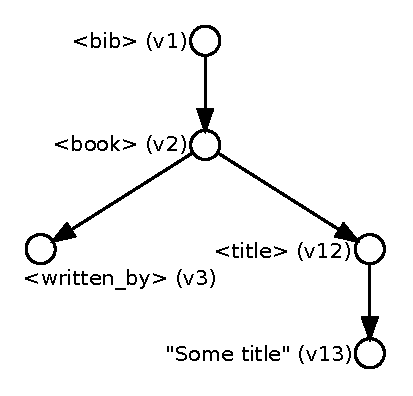
\includegraphics[scale=0.6]{nottuples2}}
	\caption[Two subtrees of the XML tree]{Two subtrees of the XML tree in Fig. \ref{example1} which are not tree tuples}
    \label{nottuples}
\end{figure}

In Fig. \ref{nottuple1}, the subtree is not a tree tuple, because the answer of the path $/bib/book/written\_by/author$ contains two distinct nodes (i.e. $v4$ and $v8$). The subtree in the Fig. \ref{nottuple2} is not a tree tuple, because it is not a maximal subtree (it is a subtree of a tuple from Fig. \ref{tuples}).\qed

\end{example}

\begin{define}[Functional Dependency]\label{fd1}
Being given a DTD $D$, a {\sl functional dependency} on $D$ is an expression of the form $S \rightarrow p$, where $S$ is a finite non empty subset of $paths(D)$ and $p \in paths(D)$.\qed
\end{define}

\begin{example}\label{fdExample}
Consider the XML tree in Fig \ref{example1}. The following functional dependency expresses the constraint that two distinct authors of the same book cannot have the same value of attribute \texttt{ano}:$$\{/bib/book, /bib/book/written\_by/author/@ano\} \rightarrow /bib/book/written\_by/author$$\qed
\end{example}

\subsection{Functional Dependency 2}

\begin{define}[Functional Dependency]\label{fd2}
With a given DTD $D$, a {\sl functional dependency} is of the form $\sigma = (P, P', (P_1, \dots, P_n \rightarrow P_{n+1}))$. Here $P$ is a  root path (path where the first element is a root element of an XML document), or $P = \epsilon$ (empty path). Each $P_i (i \in [1,n])$ is a singleton leaf path, and there is a no non-empty common prefix for $P_1, \dots, P_{n+1}$. Being given an XML document $T$ conforming to $D$, we say $T$ satisfies $\sigma$:iff $\forall v \in \{[\![P]\!]\}, \forall v_1, v_2 \in \{v[\![P']\!]\}$, if $v_1[\![P_i]\!] \equiv v_2[\![P_i]\!]$ for all $i \in [1,n]$, then $v_1[\![P_{n+1}]\!] \equiv v_2[\![p_{n+1}]\!]$.\qed
\end{define}

The main difference between two definitions of the functional dependency is that the former definition can use any path from $paths(D)$, whereas the latter considers that each $P_i (i \in [1,n])$ is from $StrPaths(D)$. That means the constraint from Example \ref{fdExample} cannot be expressed by functional dependency defined in \ref{fd2}, because of $/bib/book/written\_by/author$ path. Nevertheless, modified constraint from Example \ref{fdExample} expressed by FD defined in \ref{fd2} is shown in Example \ref{fd2Example}.

\begin{example}\label{fd2Example}
Consider the constraint $C$ saying that two distinct authors with different names of the same book cannot have the same value of attribute \texttt{ano}. The functional dependency expressing $C$ is defined as follows:

$$(bib/book, written\_by/author, (@ano \rightarrow name))$$\qed
\end{example}
